% Author: Izaak Neutelings (November 2023)
% https://cds.cern.ch/record/1019832/
% https://gitlab.cern.ch/tdr/papers/HIN-23-011/-/blob/412e731355f387f9972edcb760f077c2e6d58e84/figures/Introduction/CMS_det.png
\documentclass[border=3pt,tikz]{standalone}

% COLORS
\colorlet{colTRKR}{orange!95!black!50} % tracker
\colorlet{colECAL}{green!70!black!50}  % ECAL
\colorlet{colHCAL}{cyan!90!black!40}   % HCAL
\colorlet{colMUON}{red!80!black!40}    % MUON
\colorlet{colCSTR}{cyan!95!black!20}   % CASTOR
\colorlet{colZDC}{pink!80!magenta!90!black!60} % ZDC
\colorlet{coljet}{blue!87!red!98!black!45} % jet

% STYLES
\tikzset{>=latex} % set default arrow head as latex
\tikzstyle{subdetline}=[draw=black,thick]
\tikzstyle{dashed subdetline}=[draw=black,thin,dashed]
\tikzstyle{subdet}=[subdetline,fill=#1]

\begin{document}

% CMS DETECTOR SKETCH
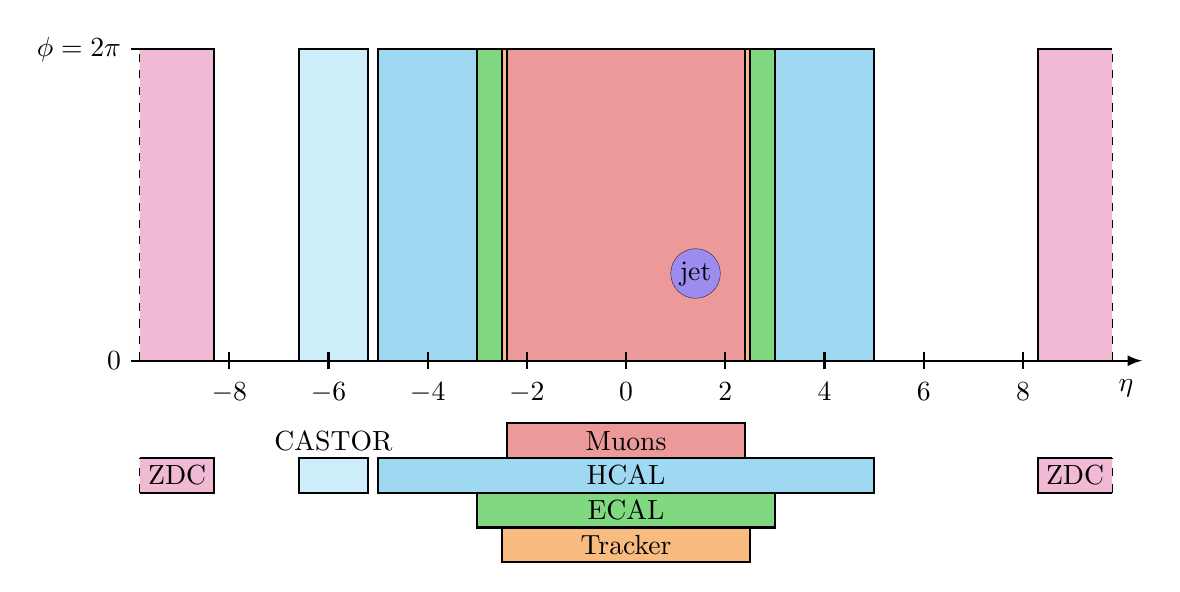
\begin{tikzpicture}[scale=0.63]
  
  % SETTINGS
  \def\hsubdet{0.7} % height subdetector
  \def\phimax{6.28} % height phi direction (2*pi)
  \def\ltick{10pt}  % tick length
  
  % PSEUDORAPIDITIES
  \def\etaTRKR{2.50}    % tracker
  \def\etaECAL{3.00}    % ECAL
  \def\etaHCAL{5.00}    % HCAL
  \def\etaMUON{2.40}    % MUON
  \def\etaminCSTR{5.20} % CASTOR
  \def\etamaxCSTR{6.60} % CASTOR
  \def\etaminZDC{8.3}   % ZDC (lower)
  \def\etamax{9.8}      % maximum eta
  
  % ETA-PHI PLANE
  \begin{scope}[shift={(0,5.8*\hsubdet)}]
    
    \fill[colZDC] % fill without line
      (-\etamax,0) rectangle (-\etaminZDC,\phimax)
      ( \etamax,0) rectangle ( \etaminZDC,\phimax);
    \draw[subdetline] % solid line
      (-\etamax,0) -| (-\etaminZDC,\phimax) -- (-\etamax,\phimax)
      ( \etamax,0) -| ( \etaminZDC,\phimax) -- ( \etamax,\phimax);
    \draw[dashed subdetline] % dashed line
      (-\etamax,0) -- (-\etamax,\phimax)
      ( \etamax,0) -- ( \etamax,\phimax);
    \fill[subdet=colCSTR]
      (-\etamaxCSTR,0) rectangle (-\etaminCSTR,\phimax);
    \fill[subdet=colHCAL]
      (-\etaHCAL,0) rectangle (\etaHCAL,\phimax);
    \fill[subdet=colECAL]
      (-\etaECAL,0) rectangle (\etaECAL,\phimax);
    \fill[subdet=colTRKR]
      (-\etaTRKR,0) rectangle (\etaTRKR,\phimax);
    \fill[subdet=colMUON]
      (-\etaMUON,0) rectangle (\etaMUON,\phimax);
    
    % PSEUDORAPITY (ETA) AXIS
    \draw[->,thick] (-\etamax,0) -- (\etamax+0.6,0)
      node[anchor=60,inner sep=6.5pt] {$\eta$};
    \foreach \e in {-8,-6,...,8}{
      \draw[thick] (\e,\ltick/2) --++ (0,-\ltick)
        node[below=1pt] {$\e$};
      %\node[below=1pt] at (\e,0) {$\e$}; % without tick
    }
    %\node[below=1pt] at (9.2,-\ltick/2) {$\eta$};
    
    % AZIMUTHAL ANGLE (PHI) TICK LABELS
    \draw[thick] (-\etamax,0)++(\ltick/2,0) --++ (-\ltick,0)
      node[left=0pt] {$0$};
    \draw[thick] (-\etamax,\phimax)++(\ltick/2,0) --++ (-\ltick,0)
      node[left=0pt] {$\phi=2\pi$};
    
    % JET CONE
    %\node[circle,draw=black,ultra thin,fill=coljet,inner sep=1.2pt]
    % at (1.4,0.28*\phimax) {jet};
    \draw[ultra thin,fill=coljet]
      (1.4,0.28*\phimax) circle(0.5)
      node[scale=1] {jet};
     
  \end{scope}
  
  % SKETCH
  \fill[subdet=colTRKR]
    (-\etaTRKR,0) rectangle (\etaTRKR,\hsubdet)
    node[midway] {Tracker};
  \fill[subdet=colECAL,shift={(0,\hsubdet)}]
    (-\etaECAL,0) rectangle (\etaECAL,\hsubdet)
    node[midway] {ECAL};
  \fill[subdet=colHCAL,shift={(0,2*\hsubdet)}]
    (-\etaHCAL,0) rectangle (\etaHCAL,\hsubdet)
    node[midway] {HCAL};
  \fill[subdet=colMUON,shift={(0,3*\hsubdet)}]
    (-\etaMUON,0) rectangle (\etaMUON,\hsubdet)
    node[midway] {Muons};
  \fill[subdet=colCSTR,shift={(0,2*\hsubdet)}]
    (-\etamaxCSTR,0) rectangle (-\etaminCSTR,\hsubdet);
    %node[midway] {CASTOR};
  \node[above=-1pt,xscale=1]
    at ({-(\etaminCSTR+\etamaxCSTR)/2},3*\hsubdet) {CASTOR};
  
  % SKETCH ZDC
  \begin{scope}[shift={(0,2*\hsubdet)}]
    \fill[colZDC] % fill-only, no line
      (-\etamax,0) rectangle (-\etaminZDC,\hsubdet)
      node[black,midway] {ZDC}
      (\etamax,0) rectangle (\etaminZDC,\hsubdet)
      node[black,midway] {ZDC};
    \draw[subdetline] % solid line
      (-\etamax,0) -| (-\etaminZDC,\hsubdet) -- (-\etamax,\hsubdet)
      ( \etamax,0) -| ( \etaminZDC,\hsubdet) -- ( \etamax,\hsubdet);
    \draw[dashed subdetline] % dashed line
      (-\etamax,0) -- (-\etamax,\hsubdet)
      ( \etamax,0) -- ( \etamax,\hsubdet);
  \end{scope}
  
\end{tikzpicture}


\end{document}